\documentclass{standalone}
\usepackage{tikz,pgfplots}
\usetikzlibrary{decorations.pathreplacing,patterns}
\pgfplotsset{compat=newest}
\begin{document}
  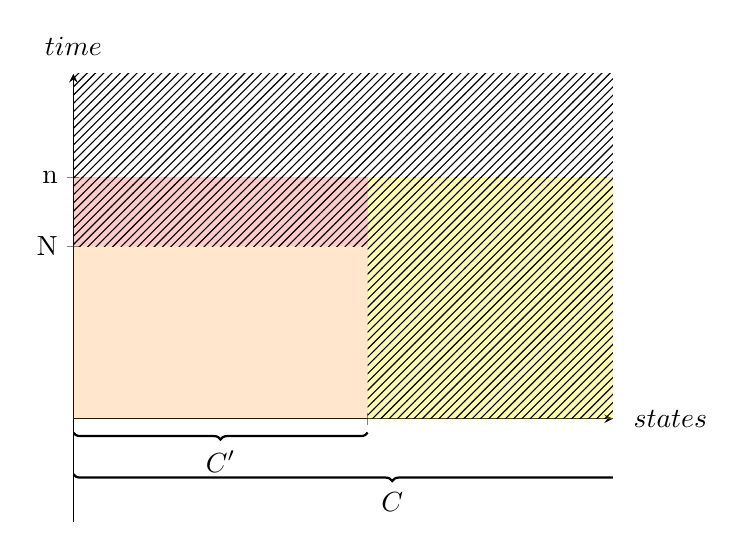
\begin{tikzpicture}
    \newcommand\n{0.7};
    \newcommand\N{0.5};
    \newcommand\Cp{0.6};

    \begin{axis}[axis lines=middle,samples=200
            ,ylabel=$time$
            ,xlabel=$states$
            ,xmax=1.1
            ,ymax=1
            ,ymin=-0.3
            ,xmin=0
            ,every axis x label/.style={
              at={(ticklabel* cs:1.02)},
                anchor=west,
              },
            every axis y label/.style={
              at={(ticklabel* cs:1.02)},
                anchor=south,
              },
            ,xtick=data,
            ,xtick={\Cp}
            ,xticklabels={}
            ,ytick=data,
            ,ytick={\N,\n}
            ,yticklabels={N,n}
            ]
            \draw [fill=orange,orange,opacity=0.2,draw=none] (0,0) rectangle (\Cp,\N);
            \draw [fill=red,red,opacity=0.2,draw=none] (0,\N) rectangle (\Cp,\n);
            \draw [yellow,opacity=0.3,fill=yellow,draw=none] (\Cp,0) rectangle (2\Cp,\n);
            \begin{scope}{on foreground layer}    % select the background layer
                \draw[pattern=north east lines,draw=none] (\Cp,0) rectangle (2\Cp,\n);
                \draw[pattern=north east lines,draw=none] (0,\N) rectangle (\Cp,\n);
            \end{scope}
            \draw[pattern=north east lines,draw=none] (0,\n) rectangle (2\Cp,2\n);
            % underbraces
            % \draw [thick, red,decorate, decoration={brace,amplitude=10pt ,mirror} ,xshift=0.4pt,yshift=-0.4pt] (0,.2) -- (\Cp,0) node[black,midway,yshift=-0.6cm] {\footnotesize $t$} ;
            \draw[decorate,decoration={brace,mirror},thick]  ([yshift=-5pt]axis cs:0,0) --    node[below=3pt] {$C^\prime$}   ([yshift=-5pt]axis cs:\Cp,0);
            \draw[decorate,decoration={brace,mirror},thick]  ([yshift=-20pt]axis cs:0,0) --    node[below=3pt] {$C$}   ([yshift=-20pt]axis cs:1.3,0);
          \end{axis}
  \end{tikzpicture}
\end{document}
